\documentclass[twocolumn]{jarticle}%,2pt
\setlength{\columnsep}{3zw} 

\title{\vspace{5mm}\large{拡張現実感技術を用いた歩行者シミュレーション}\vspace{-15mm}}
%\title{\tiny{}}
\date{}


\usepackage{textcomp}
\usepackage[sc]{mathpazo}
\usepackage[scaled]{helvet}
\usepackage{amsmath,amssymb}
%\usepackage{otf}%字体が変更できる
\usepackage{color}
\usepackage{threeparttable}
\usepackage[dvipdfmx,hiresbb]{graphicx}%
\usepackage{float}
\usepackage{fancyhdr}
\usepackage{titlesec}
\usepackage[top=30truemm,bottom=30truemm,left=20truemm,right=20truemm]{geometry}

%define for header%\titleformat*{\section}{\large\bfseries}
\titleformat*{\section}{\large\bfseries}
\renewcommand{\ttdefault}

%Header
\pagestyle{fancy}%ページ番号を入れるか決めてるっぽい.
\rhead{}
\lhead{出願区分 : 情報科学区分 \\ 氏名 : 小黒司友 \\ 現在の専門 : 情報工学 \\ 希望希望研究室: インタラクティブメディア設計学研究室}

\begin{document}
\normalsize
%\author %
\maketitle

\section{はじめに}
\thispagestyle{fancy}

私が,奈良先端科学技術大学院大学(以下NAIST)で取り組みたい研究テーマは「拡張現実感技術を用いた歩行者シミュレーション」である.本稿では,第\ref{current}章でこれまでの修学内容について,第\ref{want}章で貴学で取り組みたい研究テーマの研究背景及び目的・先行研究・提案手法について述べ,結びとする.

\section{現在行っている研究}\label{current}
私が現在行っている研究は,歩行者交通流シミュレータのための歩行モデルの検討である.その詳細を以下に述べる.

\subsection{研究背景}
これまでに,歩行者集団の移動の円滑性・効率性に着目する交通流シミュレータが開発されていた.しかし,歩行者と空間を共有するパーソナルモビリティやロボットを,安全かつ快適に運用するには,個々の歩行者の振る舞いや歩行者間の相互作用までシミュレートする必要がある.

そこで本研究では,歩行者に近い歩行ルール(歩行モデル)を持つアバターを扱うシミュレータを作成することを最終的な目標とする.

%現段階では,シミュレーション環境で各歩行モデルを用いてシミュレーションが行えることを確認した.さらに,アバター操作モードを用いて,被験者がシミュレーションに介入できることを確認した.今後は,歩行モデルとアバター操作モードを用いてシミュレーションを行った結果から,歩行モデルの評価を行う.歩行モデルの評価は,効率性\cite{Iryo-4},安定性\cite{Iryo-4},安全性,みための自然さ\cite{Iryo-2}の観点から行う.

\subsection{シミュレータ}
図\ref{fig:environment}に示すようなシミュレーション環境でシミュレーションを行う.

アバターの歩行開始地点もしくは目的地となる歩道 A,B,C,D を用意する.アバターの流れは様々に設定できるようにする.

空間を2次元平面で考え,アバターは円形領域とする. アバターの流入位置および目的地,円形領域の半径,基本的な歩行速度などは独立に一定の確率分布を与えて決定する.シミュレーションは離散時間間隔で進行させ,アバターの通し番号や座標,衝突状況などの情報をログファイルに記述する. 

また,被験者がシミュレーション中にどのような行動を行うのかをデータとして得るために,アバターのうちの一体としてアバターを操作し,シミュレーションに参加することができるモード(アバター操作モード) を用いる.ログファイルを元にシミュレーションの様子をVRビューアで可視化したうえで,被験者は,図\ref{fig:user_view}のように一人称視点でシミュレーション空間に没入しながら他のアバターの様子を観察しつつアバターの操作を行う.

\subsection{歩行モデル}
今回のシミュレータでは,3種類の性質の異なる歩行モデルを用いる.使用するそれぞれの歩行モデルについて,概要を示す.\\

モデル1 : ポテンシャルモデル\cite{Akuzawa}\\
歩行モデルに同一符号の電荷を持たせ,クーロン力により歩行モデル間の斥力を計算し,全てのアバターについて足し合わせる.さらに,目的地に向かう力を加えて最終的にアバターが受ける力を計算する. \\

モデル2 : 追従型モデル\cite{Sasagawa}\\
目的地に向かう基本的な速度 を持ち,前方に他の目的地を持つアバターがいれば回避,同一の目的地のアバターがいれば追従する付加的な速度を加える.\\

モデル3 : 効率重視型モデル\\
アバターに視野を定め,視野内の他のアバターとの衝突を避けつつ目的地に向かう方向と速度を選択する. \\

\begin{figure}[H]
    \begin{tabular}{cc}
      %---- 最初の図 ---------------------------
      \begin{minipage}[t]{0.45\hsize}
        \centering
        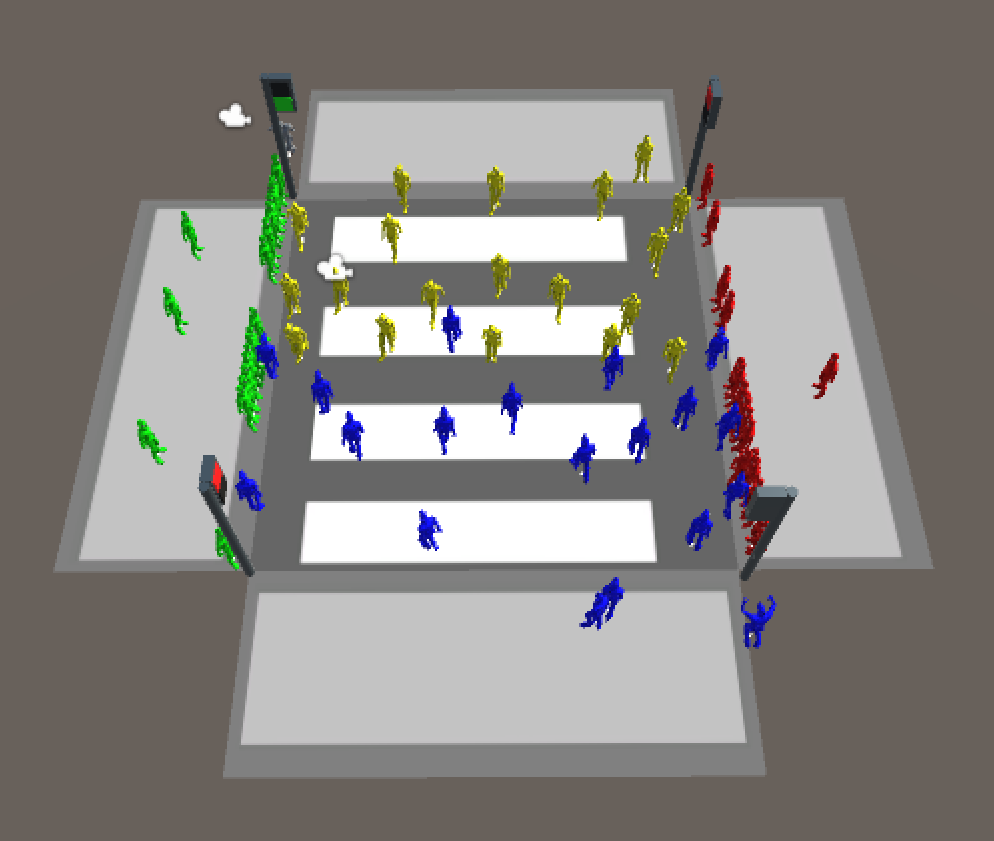
\includegraphics[keepaspectratio, scale=0.11]{images/environment.JPG}
        \caption{シミュレーション環境}
        \label{fig:environment}
      \end{minipage} &
      %---- 2番目の図 --------------------------
      \begin{minipage}[t]{0.45\hsize}
        \centering
        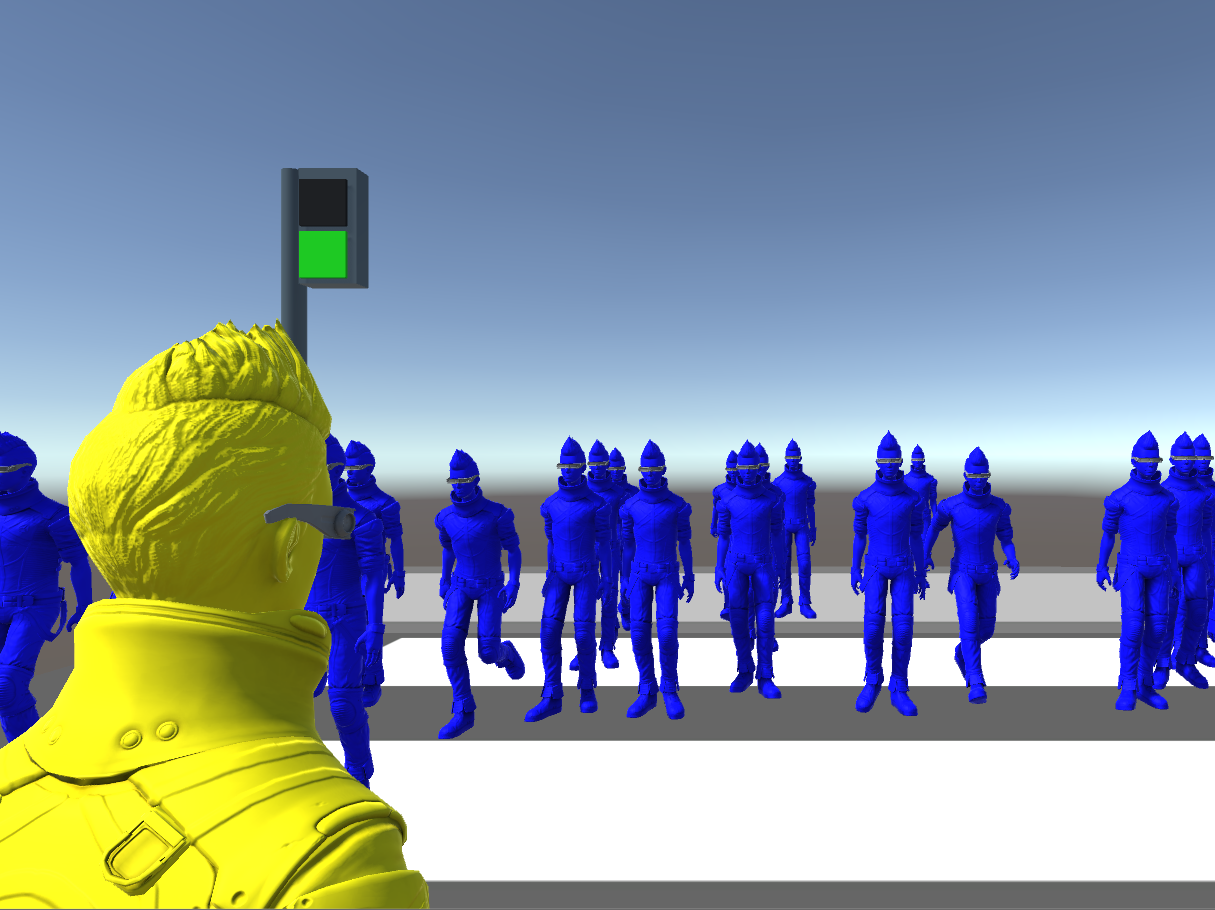
\includegraphics[keepaspectratio, scale=0.1]{images/user_view_mini.JPG}
        \caption{被験者が体験するシミュレーションの様子}
        \label{fig:user_view}
      \end{minipage}
      %---- 図はここまで ----------------------
    \end{tabular}
  \end{figure}

\section{貴学において取り組みたい研究}\label{want}
貴学では,第\ref{current}で述べた研究を基に,拡張現実感技術を用いた歩行者シミュレーションについて研究したいと考えている.

%第\ref{current}でも述べたように,
個々の歩行者の振る舞いや歩行者間の相互作用注目したシミュレーションにおいては,安全性や人間らしさといった評価の観点を欠かすことができない.

その評価手法として,仮想空間を歩行者として体験することのできる,バーチャルリアリティ(VR)型のシミュレータが提案されている\cite{Iryo-1},\cite{Iryo-2},\cite{Iryo-3}.

しかし,現実の環境を想定したシミュレーションを行うことが難しいという問題がある.また,人間の主観を用いた評価の特性上,現実の環境ではないことが評価に影響を与えてしまうことも考えられる.

そこで,拡張現実感技術(AR)を用いて,現実空間での歩行者シミュレーションを行う.

図\ref{fig:systemImage}にシステムの概要図を示す.
システムは,歩行者シミュレーションを行うためのシミュレータ,歩行者シミュレーション結果を描画指示する描画指示部(ビューア),実際にシミュレーションの様子を描画するARヘッドマウントディスプレイ(HMD)デバイスで構成される.

シミュレータでシミュレーション環境を設定したうえで,微小時間ごとにアバターを歩行モデルに従って移動させる.微小時間ごとに変化するアバターの座標や,アバターの発生・消滅指示,描画についての指定などの情報を,ソケット通信することでビューアに対して伝える.

ビューアは,通信で受け取った情報をもとに,歩行者シミュレーションの様子をARHMDに対して描画する.

ユーザは,ARHMDに描画される歩行者シミュレーションの様子を観察しながら,アバターのうちの一体として歩行しながら目的地を目指す.
ビューアは,シミュレーション環境中のユーザの座標をシミュレータとソケット通信することで伝達する.
シミュレーション空間中のユーザの座標は,ARHMDのカメラと深度センサを使った3Dマッピングによって求める.

\begin{figure}[htbp]
  \begin{center}
    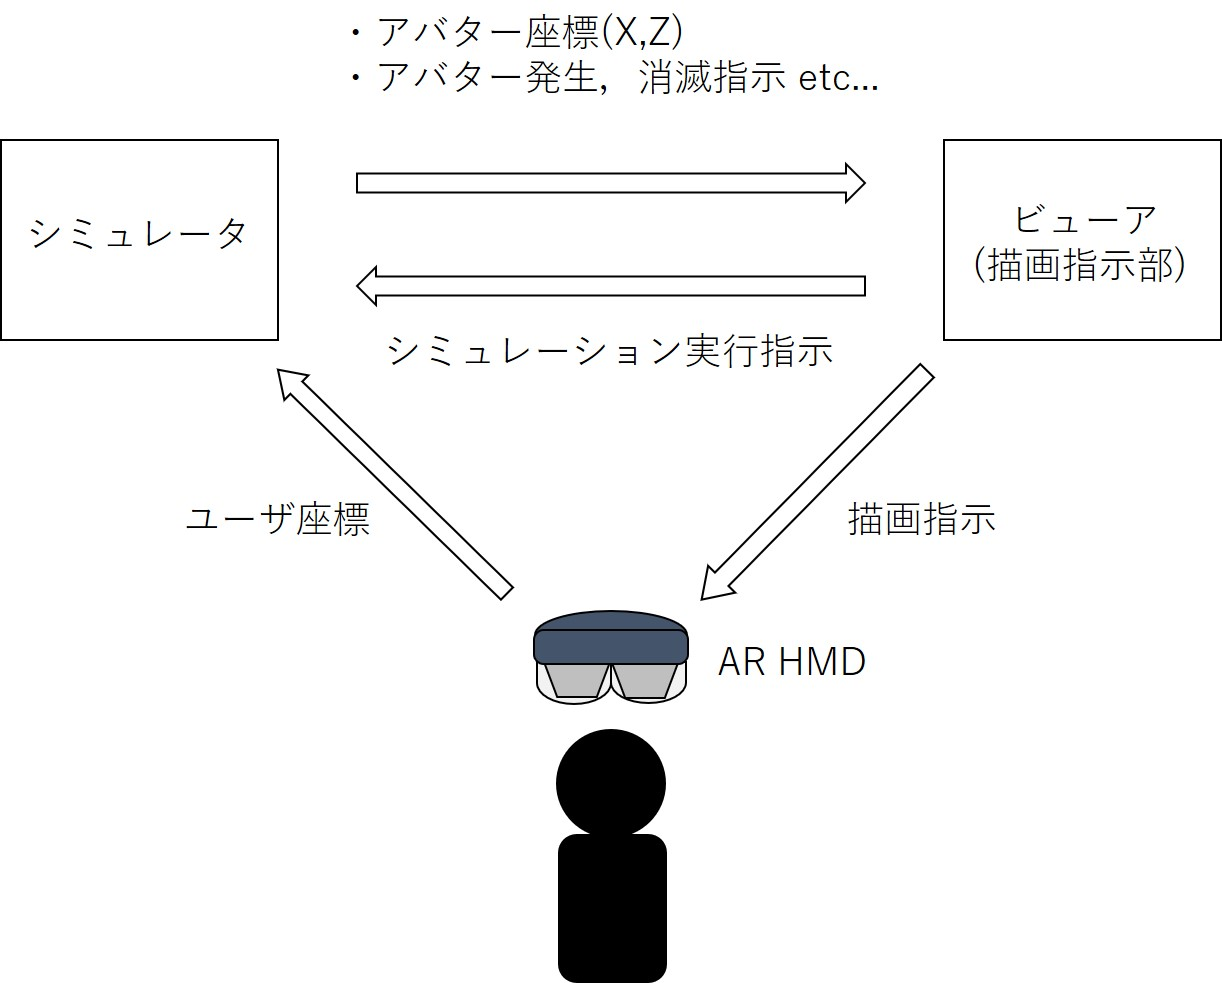
\includegraphics[width=80mm]{images/systemImage.jpg}
  \end{center}
    \caption{システム概要図}
    \label{fig:systemImage}
\end{figure}

\section{おわりに}
本稿では,現在取り組んでいる研究についてと,貴学で取り組みたい研究について述べた.
この研究によって,歩行モデルの人間らしさに関するより現実に即した評価を実現することができる.
この研究を実現するためには,映像データの解析や,3Dマッピング技術,コンピュータビジョンに加え,ヒューマンコンピュータインタラクションなどの技術の習得が必要である.

志望するインタラクティブメディア設計学研究室では,拡張現実感技術,それらを実現するためのコンピュータグラフィックス,コンピュータビジョン,ヒューマンコンピュータインタラクションなどの研究が盛んに行われており,提案する研究テーマを取り組むために最適な環境である.

よって,私は貴学に入学し,インタラクティブメディア設計学研究室で研究することを希望する.

%参考文献
\begin{thebibliography}{1}
\bibitem[1]{Iryo-1} Miho Iryo-Asanoa,Yu Hasegawa,Charitha Dias,
``Applicability of Virtual Reality Systems for Evaluating Pedestrians’ Perception and Behavior''
 (2018)
\bibitem[2]{Iryo-2} Yu HASEGAWA, Miho IRYO-ASANO
``Development of Pedestrian Model for Experiments in Virtual Reality Environment'' (2018)
\bibitem[3]{Iryo-3} Takamasa Iryoa,MihoAsano,Shinta Odani,Shogo Izumi
``Examining factors of walking disutility for microscopic pedestrian model - A virtual reality approach'' 
(2013)
\bibitem[4]{Iryo-4} 井料美帆, 長島愛,
``歩行者交差交通流の性能評価に関する研究''
(2015)
\bibitem[5]{Akuzawa} 阿久澤あずみ
``駅構内における群衆歩行シミュレーションモデルの研究''
\bibitem[6]{Sasagawa} 笹川匠也
``人工現実感を用いた横断歩道における歩行者交通流シミュレータの開発''
\end{thebibliography}

\bibliographystyle{jplain}
\bibliography{Untitled}

\end{document}
